%%%%%%%%%%%%%%%%%%%%%%%%%%%%%%%%%%%%%%%%%%%%%%
\section{Beamline instrumentations}
\label{sec:beaminstruments}

The H4 beamline will be instrumented with a number of detectors to provide information about the beam profile, position, momentum, and particle identification. A number of proposals are being evaluated for NP02 and NP04. In this section, some of the detector options are presented.

\subsection{Particle identification}
The H4 beamline is capable of delivering two types of beam: electron and hadron beams. While the electron beam is relatively pure, the hadron beam consists of a mixture of electron, pion, kaon, and proton. Therefore it is essential to have efficient particle identification system to cleanly tag particle types on a particle by particle basis. To achieve this goal, a particle identification system based on a combination of threshold Cherenkov counters and Time-of-flight system are being considered for ProtoDUNES.

\subsubsection{Threshold Cherenkov counter}
The threshold Cherenkov counters have been used extensively in beamline to discriminate particles. Figure~\ref{fig:ckv} shows one of the counters used in the CERN test beam area. It consists of a gas radiator that is contained in a long cylindrical tube, and a detection box in which the Cherenkov light is reflected by a 45$^\circ$ mirror and focused onto a photomultiplier tube. The diameter of the cylindrical tube is designed to allow the counter to pass through the standard CERN beam pile of about 20cm. A variety of gasses (e.g. CO2, nitrogen, argon, Freon 12, air, etc.) are available at CERN to optimize particle identification. The CERN beam group plans to install one thereshold Cherenkov counter in the H4 beamline. A second counter may be added to the beamline if additional funding is available.
\begin{cdrfigure}[CERN threshold Cherenkov counter]{ckv}{CERN threshold Cherenkov counter}
  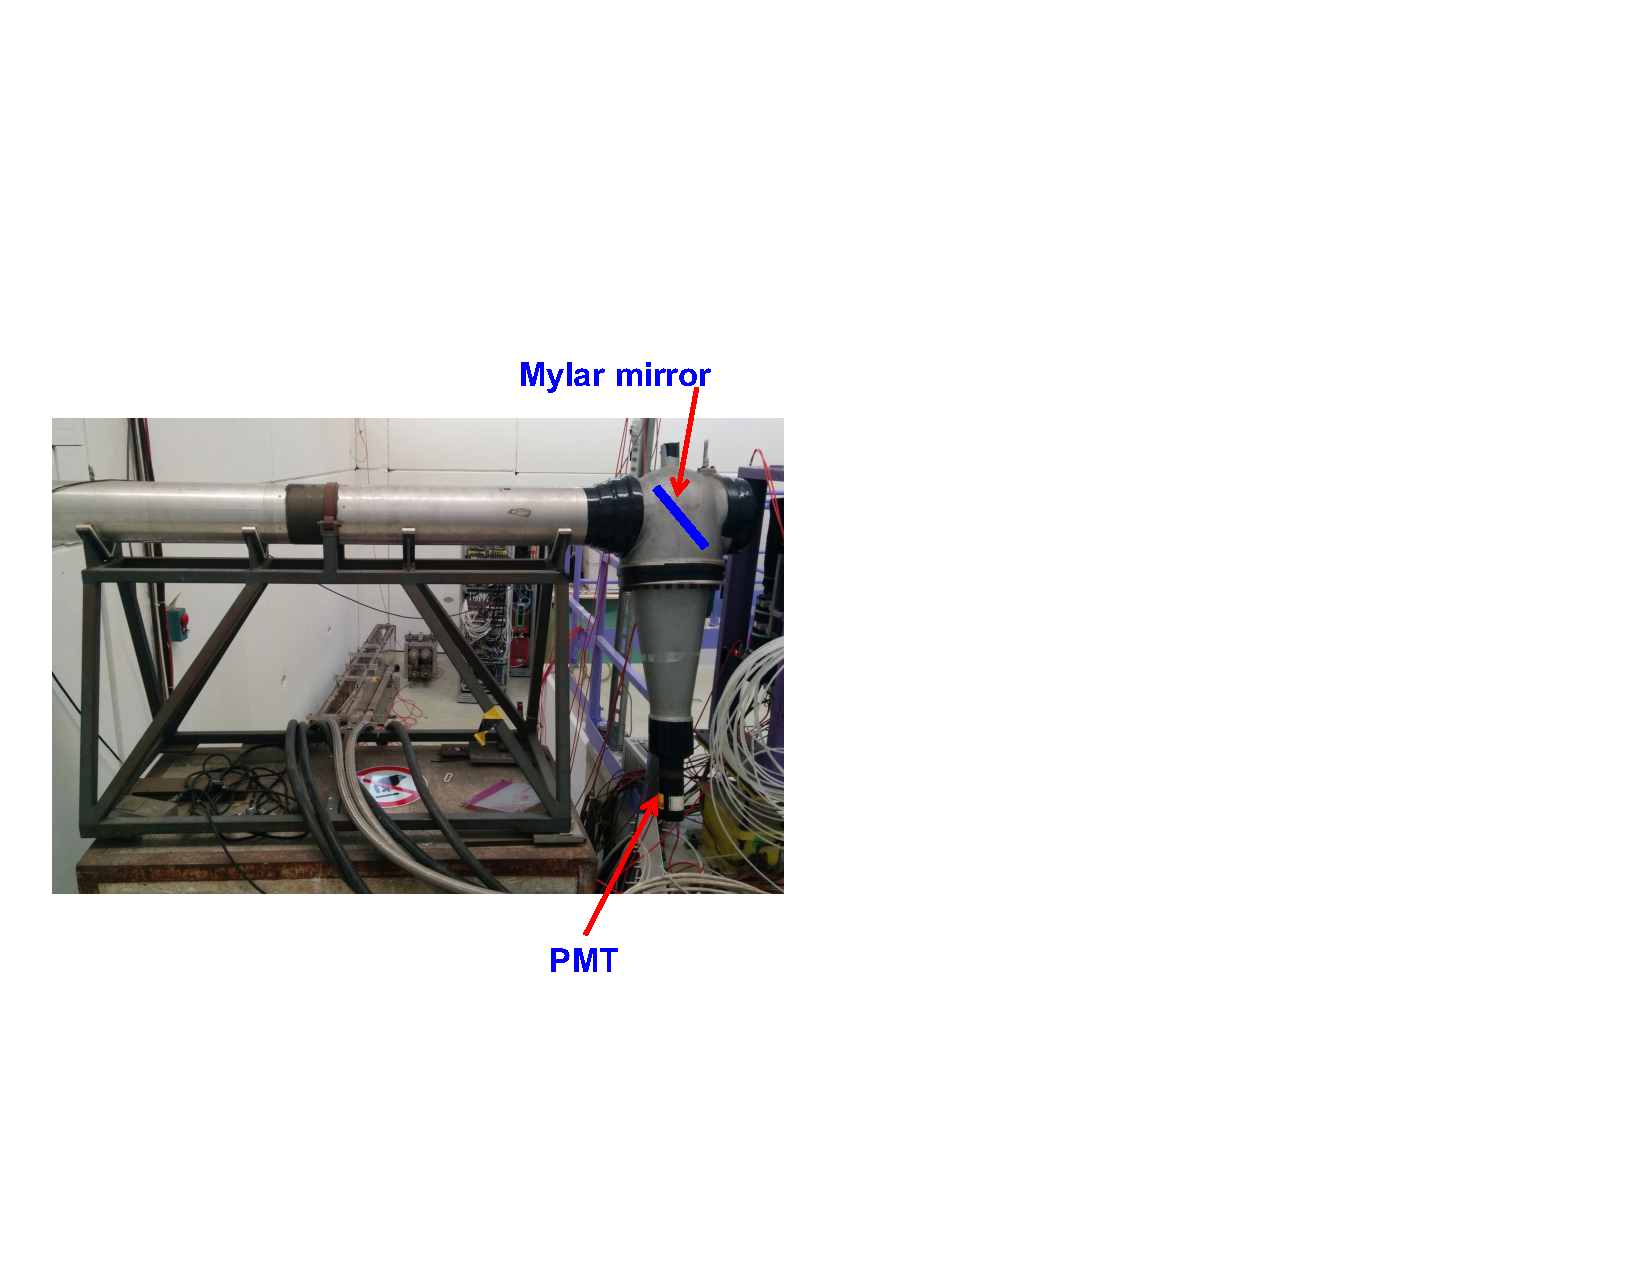
\includegraphics[width=0.65\textwidth]{beamline_ckv.pdf}
\end{cdrfigure}


\subsubsection{LAPPD Time-of-flight system}

\subsubsection{Other Time-of-flight system}

\subsection{Beam profile and particle tracking}

\subsubsection{Fiber tracker}

\subsubsection{Multiwire Proportional Chambers}

\subsection{Momentum measurements}

\subsubsection{Spectrometer}

\subsubsection{Beam collimation}

\subsection{DAQ and Trigger}

\subsubsection{Interface with artDAQ}

\subsubsection{Interface with Trigger Board}





